% !TeX root = ../main.tex

\chapter{电学性质简介}

\section{能带理论}

固体的电学性质(即电子学性质)是从能带理论出发讨论的:在固体中,大量的分子(或原子)堆积在一起,复杂而繁多的分子轨道(或原子轨道)相互作用会形成不同的\textit{能态}。能态的完整光谱带称为\textit{能带}。

在一个能带中,能态不是均匀分布的。状态函数$n(E)$定义为在$E$和$E+\delta$之间的$E$的能态个数,态密度图($E-N$图)可以很好地显示能带结构。

根据能带分布和电子填充的不同,能量有不同的性质和名称:充满电子的能带称为满带,能级最高的满带称为价带;没有电子的能带称为空带,能级最低的空带称为导带\footnote{注:不同文献对导带的定义不同,也有文献称部分充满电子的能带为导带};仅部分充满电子的能带称为部分充满能带;能级之间不能被电子填充的区域称为禁带(又称禁带,记作$Eg$)。 $0K$时,电子从最低能级开始一一填满,电子占据的最高能级称为费米能级。

绝缘体只有满带和空带(导带与价带分开),$Eg$很宽($\geq 5eV$)。在一般电场条件下,价带的电子很难激发到导电状态,电子运动状态不能改变,所以不能导电。其状态密度图如下图(c)所示;半导体也只有满带和空带(导带和价带是分开的),但Eg很窄($\leq 3eV$),在一定的电场激发下可以导电。其状态密度如下图(d)所示;导体能带的结构分为两种:一种是自身就存在的部分填充的能带(直接由分子轨道或原子轨道相互作用形成而非两能带作用形成),另一种部分填充的能带由其空带、满带重叠形成,如下图(a)(b)所示。前一种导体典型的有金属钠和金属铜,后一种导体典型的有金属钙和金属锌。

\begin{figure}
    \centering
    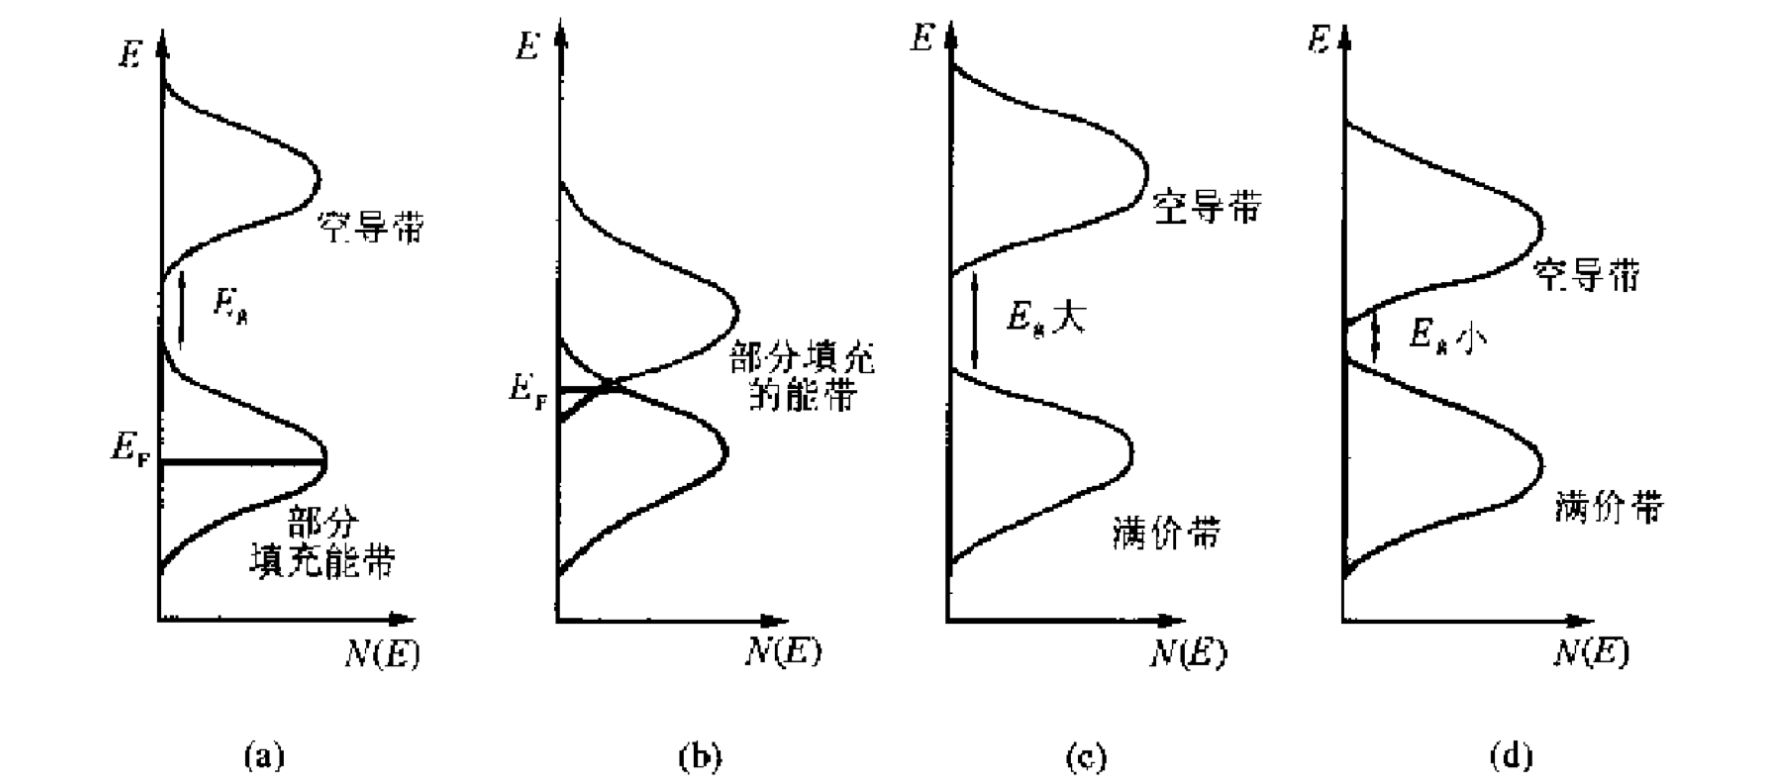
\includegraphics[scale=0.3]{img/能带.png}
    \caption{能带图像}
\end{figure}

\section{能带的直观表示方法}

叙述一下能带的直观表示方式,主要有两种:能带结构图和态密度图。态密度图的定义和举例前已叙述,实际应用中也常见态密度图的横纵坐标与前述交换;根据态密度图可以分析能隙特性。

而能带结构图纵坐标仍为能量,横坐标则为根据对称性选出的点;由于晶体的周期性,薛定谔方程的解也具有周期性,从而能带结构图可以研究整个体系各个点的能量。通过能带结构图,可以判断直接带隙或间接带隙,观察带隙、价带顶与
导带底能量。

\begin{figure}
    \centering
    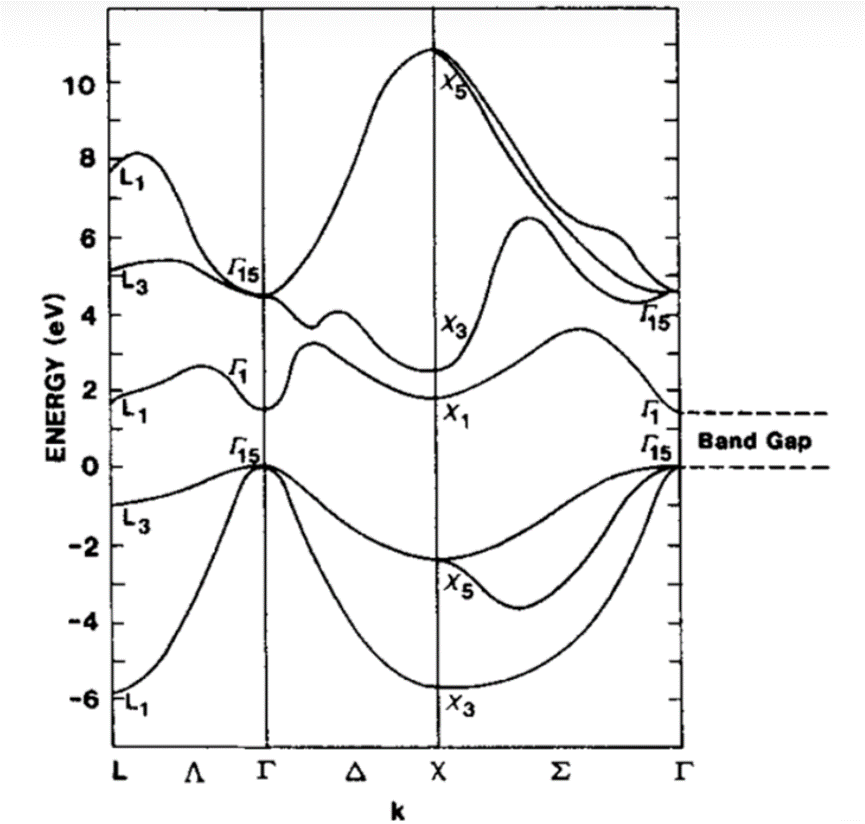
\includegraphics[scale=0.5]{img/能带结构图.png}
    \caption{能带结构图}
\end{figure}

\section{半导体的导电机制}

现重点介绍半导体的导电机制:少量电子激发至空带中后可以导电;同时,电子离开价带后会产生空穴(记为$\bigoplus$),电子运动空穴状态也会发生变化,因此空穴也可以导电(或直接将空穴视为载流子)。
本征半导体中的自由电子和空穴一样多,其状态密度如下图(a)所示。当半导体晶体掺杂杂原子时,会导致能态的变化:当掺杂价电子较多的原子时,这些电子占据导带中能量最低的电子供体能级,称为n型半导体,状态密度图如下图(b)所示;当掺杂价电子较少的原子时,在价带旁边形成空穴能级(带正电的受体能级),称为p型半导体,状态密度图如下图(c)所示。在能态发生非常小的变化后,半导体的电导率将增加几个数量级。

\begin{figure}
    \centering
    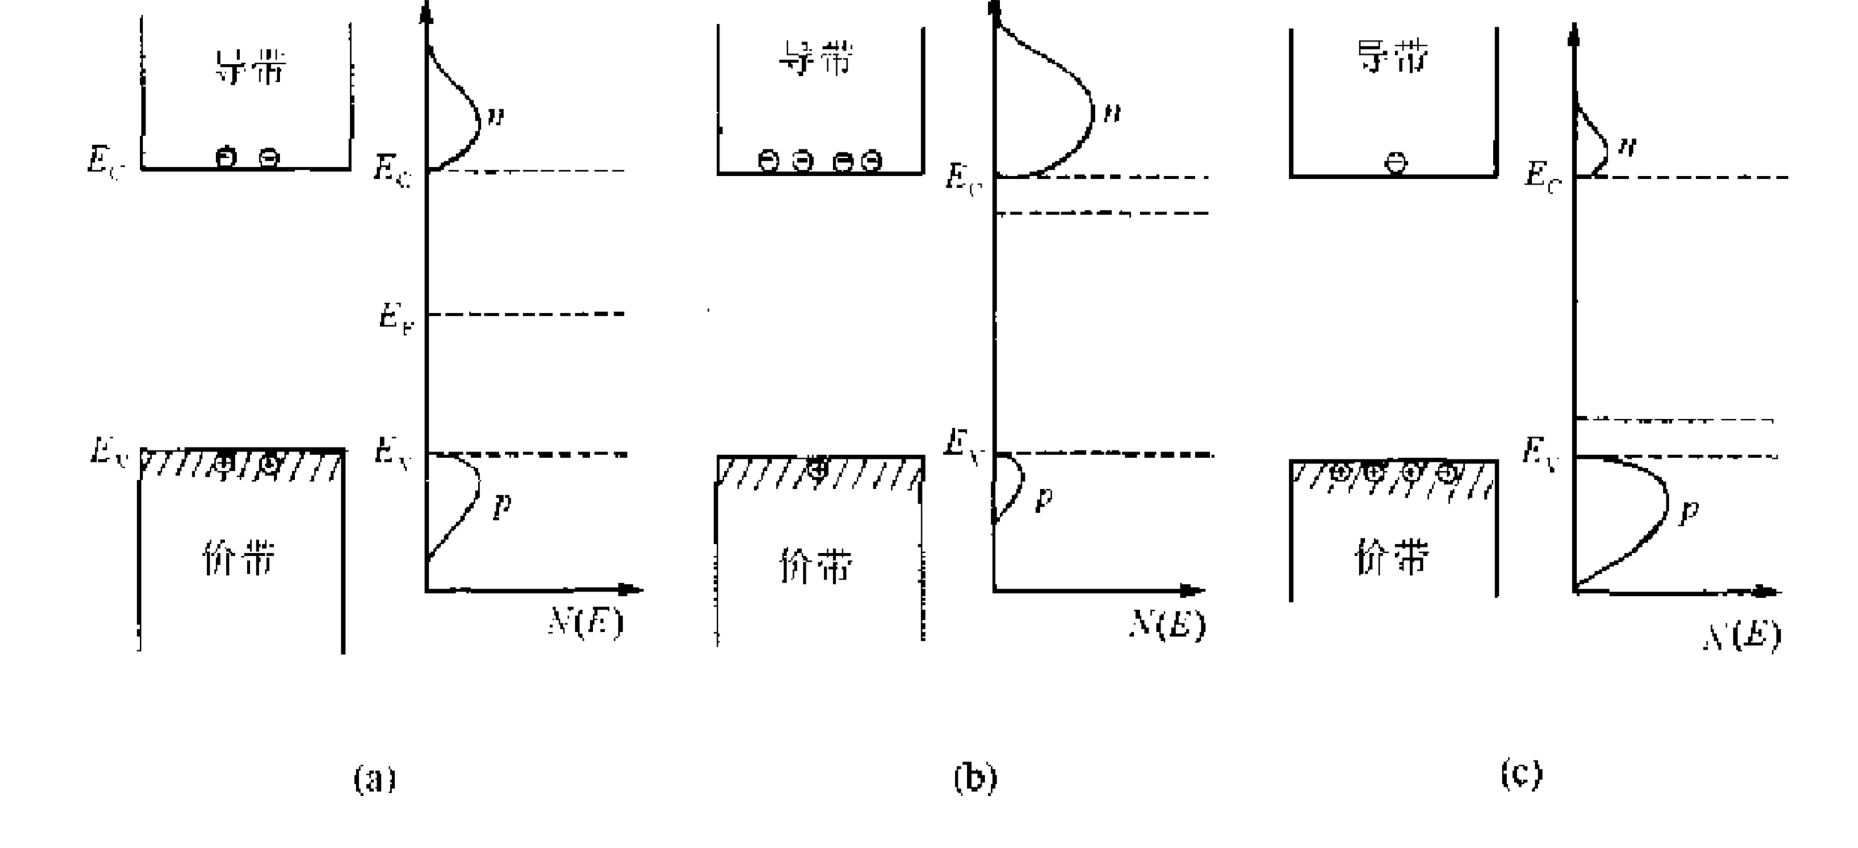
\includegraphics[scale=0.25]{img/能带示意图.png}
    \caption{能带示意图}
\end{figure}

p-n结由p型半导体和n型半导体组成;电子从n型区迁移到p型区,形成无载流子的空间电荷区域;离子化杂质的不平衡电荷导致能带弯曲,直到费米能级相等。
二极管中p-n结可用于单向导通的机理如下:载流子的消耗有效地形成绝缘势垒;如果正电位接p端,则n端比p端更负,势垒下降,载流子通过;如果n端接正电位,则更多载流子被除去,势垒变大,电阻很大(电流很小)。\cite{RN47}